% !TeX root = ../main.tex
\chapter{Prototyping and Development}
\label{chap:prototyping-dev}

\section{Introduction}


\section{Testing the LTC2945}
    The LTC2945 testing was carried out using a Linear Tech eval board, DEMO CIRCUIT 1697A. Connections and modifications were made as follows:
    \begin{itemize}
        \item VIN: tied to Arduino +5V
        \item GND: tied to Arduino GND
        \item ADIN: Tied to GND
        \item SCL: Tied to Arduino Pin D8 I2C2 SCL
        \item SDAI/SDAO (JP2 set to TIE): Arduino Pin D9 I2C2 SDA
        \item VPU: Tied to Arduino +3v3
        \item VOUT: Float or tied to dummy load (1k$\Omega$ to 10k$\Omega$)
        \item 20m$\Omega$ shunt replaced with 17$\Omega$ shunt for testing with $\sim$5k$\Omega$ load
        \item Installed 4.7k$\Omega$ pull up on I2C lines via R4, R5 footprints on EVB
    \end{itemize}

    \newpage
    \subsection{Calculating Shunt Value for Test}
    Using the 5V from the arduino as a source, and a load ranging 1k to 10k ohms, we calculate:
    $$R_{L,min}=1k\Omega$$
    $$V_{shunt}=V_S\frac{R_S}{R_L+R_S}$$
    $$R_S=\frac{V_{Shunt}R_L}{V_s-V_{Shunt}}$$
    $$V_{shunt}=0.1024V$$
    $$R_{S,full scale}=\frac{(0.1024V)(1k\Omega)}{5V-0.1024V}=20.91\Omega$$
    Adding some headroom, say, 15\%, and going to an E96 resistor value...
    $$R_S=0.85(20.91)=17.8\Omega$$
    Verifying for the high end of the range:
    $$I_{min}=\frac{5V}{10k\Omega + 17.8\Omega}=499.1\mu A$$
    $$V_{shunt, min}=(499.1\mu A)(17.8\Omega)=8.88mV$$
    The shunt will range from 8.88mV to 87.44mV, within the ADC's usable range of 0V to 102.4mV.

    \newpage
    \subsection{Pictures of Evaluation Board, Display, and Phoebus Panels}
    \begin{figure}[H]
        \centering
        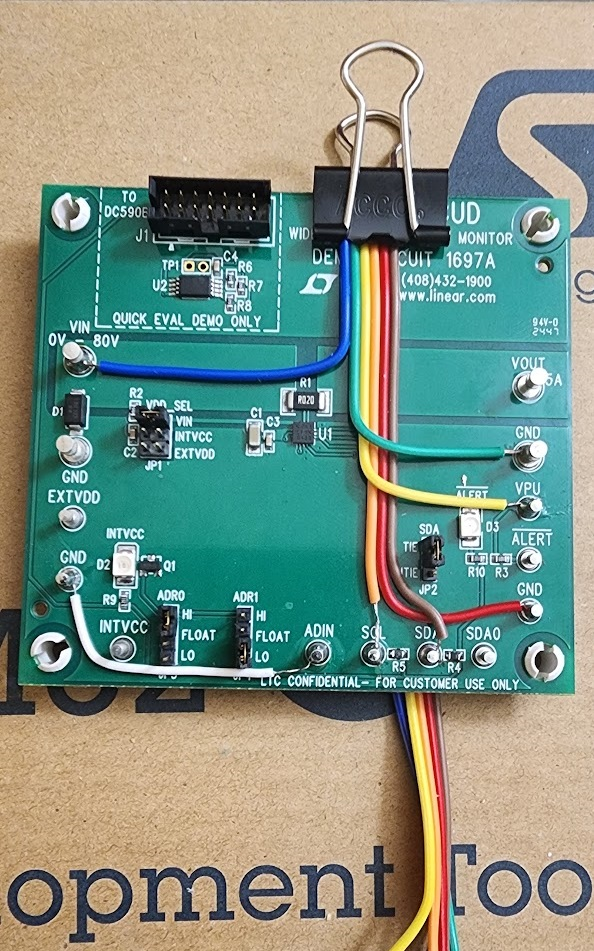
\includegraphics[
        width=3.5in,
        %height=0.85\textwidth,
        keepaspectratio
        ]{Pictures/LTC2945_EVB_Original_Shunt}
        \caption{DEMO CIRCUIT 1697A Eval Board with Original Shunt, fly leads to connect to Arduino.}
    \end{figure}

    \begin{figure}[H]
        \centering
        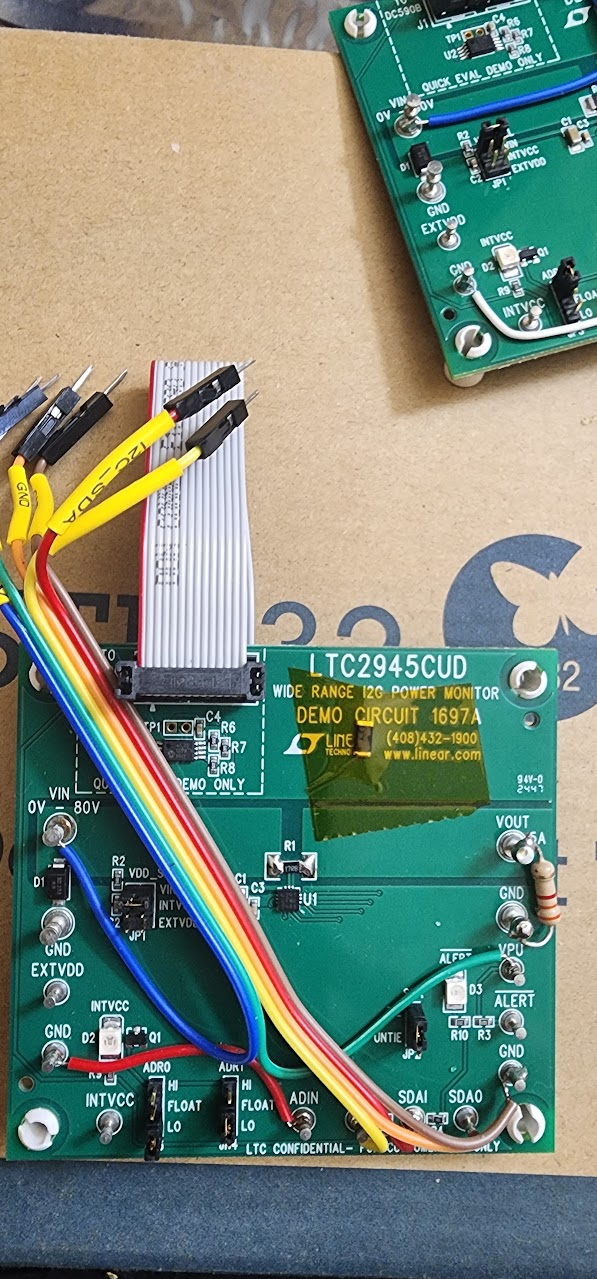
\includegraphics[
        width=3.5in,
        %height=0.85\textwidth,
        keepaspectratio
        ]{Pictures/LTC2945_EVB_17Ohm_Shunt}
        \caption{DEMO CIRCUIT 1697A Eval Board with 17$\Omega$ Shunt, fly leads to connect to Arduino, and 4.7k$\Omega$ test load.}
    \end{figure}

    \begin{figure}[H]
        \centering
        \includegraphics[
        width=3.5in,
        %height=0.85\textwidth,
        keepaspectratio
        ]{Pictures/ExampleDisplay-Single\_EVB_Connected\_Non-ALM}
        \caption{Arduino Giga with GIGA DISPLAY SHIELD showing dummy -5V rail being monitored, without alarm}
    \end{figure}

    \begin{figure}[H]
    \centering
    \includegraphics[
    width=3.5in,
    %height=0.85\textwidth,
    keepaspectratio
    ]{Pictures/ExampleDisplay-Single\_EVB_Connected\_ALM}
    \caption{Arduino Giga with GIGA DISPLAY SHIELD showing dummy -5V rail being monitored, with UVL alarm, other channels I2C ALARM.}
    \end{figure}

    \begin{figure}[H]
        \centering
        \includegraphics[
        width=3.5in,
        %height=0.85\textwidth,
        keepaspectratio
        ]{Pictures/ExampleDisplay-Single\_EVB\_Connected\_Non-ALM-3k3Load}
        \caption{Arduino Giga with GIGA DISPLAY SHIELD showing dummy -5V rail being monitored, without alarm, 3.3k$\Omega$ Load}
    \end{figure}

    \begin{figure}[H]
        \centering
        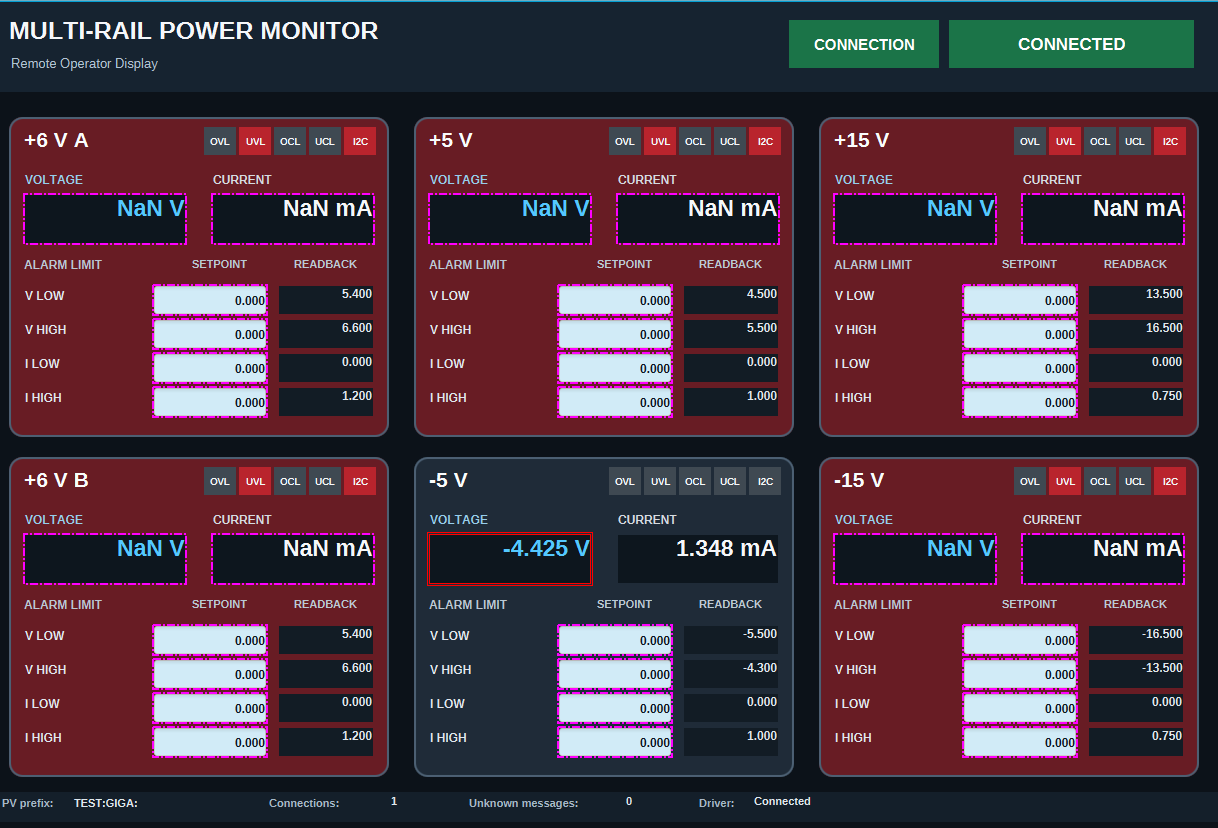
\includegraphics[
        width=\textwidth,
        %height=0.85\textwidth,
        keepaspectratio
        ]{Pictures/Phoebus-SS-N5V-Test-3k3Load}
        \caption{Arduino Giga with GIGA DISPLAY SHIELD showing dummy -5V rail being monitored, without alarm, 3.3k$\Omega$ Load}
    \end{figure}